\documentclass[border=0.3cm]{standalone}
\usepackage{tikz}
\usetikzlibrary{positioning}
\usetikzlibrary{arrows}
\begin{document}

\tikzset{%
  every neuron/.style={
    circle,
    draw,
    minimum size=0.5cm,
    fill=gray!60
  },
  neuron missing/.style={
    draw=none, 
    fill=none,
    scale=2,
    text height=0.333cm,
    execute at begin node=\color{black}$\vdots$
  },
}

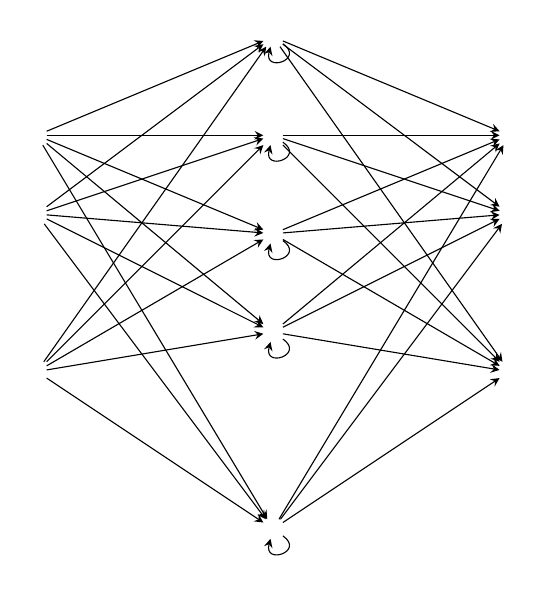
\begin{tikzpicture}[x=1.0cm, y=1.0cm, >=stealth]

\foreach \m/\l [count=\y] in {1,2,missing,3}
  \node [every neuron/.try, neuron \m/.try] (input-\m) at (0,0.5-\y) {};

\foreach \m [count=\y] in {1,2,3,4,missing,5}
  \node [every neuron/.try, neuron \m/.try] (hidden-\m) at (3,2-\y*1.25) {};

\foreach \m [count=\y] in {1,2,missing,3}
  \node [every neuron/.try, neuron \m/.try ] (output-\m) at (6,0.5-\y) {};


\foreach \i in {1,...,3}
  \foreach \j in {1,...,5}
    \draw [->] (input-\i) -- (hidden-\j);

\foreach \i in {1,...,5}
  \foreach \j in {1,...,3}
    \draw [->] (hidden-\i) -- (output-\j);

\foreach \j in {1,...,5}
  \draw [->] (hidden-\j) to [out=-35,in=-105,loop,looseness=5.5] (hidden-\j);

\end{tikzpicture}

\end{document}